\documentclass[11pt,a4paper]{article}
\usepackage[utf8]{inputenc}
\usepackage[francais]{babel}
\usepackage[T1]{fontenc}
\usepackage{amsmath}
\usepackage{amsfonts}
\usepackage{amssymb}
\usepackage{graphicx}
\usepackage{wrapfig}
\usepackage[left=2cm,right=2cm,top=2cm,bottom=2cm]{geometry}
\author{Théophile \textsc{Bastian}, Noémie \textsc{Cartier}, Nathanaël \textsc{Courant}}

\usepackage{my_listings} % On aura besoin de mettre du code source, sûrement.
% Contient \lstbash{}, \lstocaml{}, \lstc{}, ... pour mettre du code inliné facilement

\usepackage{my_hyperref} % Hyperref (pour les URLs, hyperliens, ... cliquables et colorés non-dégueulassement)

\newcommand{\htodo}[1]{\begin{huge}\colorbox{yellow}{\textcolor{red}{\textbf{TODO~:} #1}}\end{huge}}
\newcommand{\todo}[1]{\colorbox{yellow}{\textcolor{red}{\textbf{TODO~:} #1}}}
\newcommand{\relire}{\colorbox{orange}{\textcolor{blue}{\textbf{RELIRE}~}}}
\newcommand{\relu}[1]{\colorbox{green}{\textcolor{red}{\textbf{RELU~:} #1}}}
%TODO pour le rendu, supprimer ces commandes et recompiler pour s'assurer de ne pas avoir laissé de TODO

\title{Rapport de projet -- Système digital}
\date{24 janvier 2016} % Date de rendu
\begin{document}
\maketitle

\htodo{Se décider sur la typographie~: ALU ou \textsc{alu}~?}

\todo{Idem pour RAM/\textsc{ram}, ROM/\textsc{rom}, ...}

\relire
\relu{No}
\begin{abstract}
Notre objectif dans ce projet a été principalement d'avoir un code \emph{correct} et \emph{rapide à l'exécution}~; nous pensons avoir atteint ces deux objectifs. Dans ce but, nous avons commencé par implémenter non pas un simulateur, mais un \emph{compilateur} de netlists~; puis avons produit un code assembleur pour l'horloge extrêmement optimisé, tout en conservant un nombre constant de cycles processeur par incrément de seconde. Notre processeur en lui-même s'inspire fortement d'une architecture ARM, sans toutefois rechercher l'exhaustivité des opérations, ce qui nous a permis d'obtenir un processeur fonctionnel et composé de peu de portes, donc efficace. Pour finir, nous avons implémenté une GUI affichant un écran composé de blocs 7 segments, contrôlés directement par la sortie du processeur, optimisée jusqu'à ce que le programme limitant la vitesse d'exécution soit le processeur lui-même.

En définitive, les programmes obtenus, une fois combinés correctement, répondent bien au cahier des charges imposé et permettent d'atteindre une vitesse d'exécution en mode \textit{fast} de l'ordre de \textbf{9.25 jours simulées par seconde réelle}.
\end{abstract}

\setcounter{tocdepth}{2} % Limite la TOC à sections/subsections
\tableofcontents
\pagebreak


%%%%%%%%%%%%%%%%%%%%%%%%%%%%%%%%%%%%%%%%%%%%%%%%%%%%%
\section{Utilisation globale}
%%%%%%%%%%%%%%%%%%%%%%%%%%%%%%%%%%%%%%%%%%%%%%%%%%%%%

\todo{abstract ?}
\relire
\relu{Nathanaël}
\relu{No}

\subsection{Utilisation}

La compilation de toutes les composantes du projet s'effectue simplement par un \lstbash{make} à la racine du projet. Les dépendances suivantes sont toutefois nécessaires~:

\begin{itemize}
\item OCaml~: \lstbash{ocamlbuild}, \lstbash{ocamlopt}, \lstbash{ocamllex}, \lstbash{menhir}~;
\item C~: \lstbash{gcc}~;
\item C++~: \lstbash{g++}~;
\item Python~: \lstbash{python3}~;
\item Qt version $\geq 4$, \lstbash{qmake}~;
\item un environnement bash.
\end{itemize}

Le lancement de l'horloge peut se faire dans trois modes~:
\begin{itemize}
\item temps réel~: \lstbash{make run} ou \lstbash{./run_realtime.sh}, horloge en temps réel synchronisée sur le temps système à l'initialisation~;
\item rapide~: \lstbash{make run-fast} ou \lstbash{./run_fast.sh}, horloge en accéléré initialisée sur le temps du système~;
\item rapide, initialisé à 0~: \lstbash{./run_fast_0.sh}, horloge en accéléré initialisée au 1er janvier 0000, \verb!00:00:00!, utile pour évaluer la performance.
\end{itemize}

\subsection{Organisation du projet}

Les éléments du projet sont répartis dans des dossiers comme il suit~:
\begin{itemize}
\item \texttt{assembler}~: l'assembleur pour notre processeur (§\ref{sec:cas})~;
\item \texttt{clock}~: les codes assembleur de nos programmes d'horloge et nos quartz (§\ref{sec:clock})~;
\item \texttt{display\_gui}~: l'interface d'affichage (§\ref{sec:gui})~;
\item \texttt{processor}~: le code produisant la netlist de notre processeur (§\ref{sec:proc})~;
\item \texttt{simulator}~: le compilateur de netlists (§\ref{sec:compilo}).
\end{itemize}

%%%%%%%%%%%%%%%%%%%%%%%%%%%%%%%%%%%%%%%%%%%%%%%%%%%%%
\section{Compilateur de netlists} \label{sec:compilo}
%%%%%%%%%%%%%%%%%%%%%%%%%%%%%%%%%%%%%%%%%%%%%%%%%%%%%

\todo{Abstract}

\todo{Euh, je mets quoi dans l'abstract~?}

\relire
\relu{Nathanaël}
\relu{No}

\subsection{Utilisation}

Pour compiler le compilateur, il suffit de faire
\lstbash{ocamlbuild compiler.native} dans le dossier du simulateur
(\verb!simulator!), ou un simple \lstbash{make} dans le dossier du
projet.

L'utilisation du compilateur est la suivante~:

\lstbash{./compiler.native [options] fichier.net}

Le compilateur produira un fichier C \verb!fichier.c!, et un fichier
éxécutable \verb!fichier!. Les options acceptées sont les suivantes~:
\begin{itemize}
\item{\verb!-print!~: n'écrit que le code C, en particulier, ne
    produit pas l'éxécutable \verb!fichier!~;}
\item{\verb!-iomode!~$n$~: choisit le mode d'entrée-sortie de la
    netlist compilée. Les modes d'entrée-sortie sont les suivants~:
    \begin{itemize}
    \item{0~: entrées-sorties interactives, les nappes de fils étant
        considérées comme des entiers 64 bits non signés, qui sont
        affichés et demandés à l'utilisateur en décimal. C'est la
        valeur par défaut~;}
    \item{1~: chaque bit d'entrée-sortie est représenté par un
        caractère \verb!'0'! ou \verb!'1'!~;}
    \item{2~: chaque nappe d'entrée-sortie est représentée de la
        manière la plus compacte possible sur un nombre entier de
        caractères, dans l'ordre \textit{big-endian}~;}
    \end{itemize}
}
\item{\verb!-n!~$n$~: nombre de cycles à simuler. Si $n$ est omis, il
    est pris comme égal à $+\infty$.}
\end{itemize}

Le fichier éxécutable produit prend autant d'arguments que le nombre
de \textsc{rom}s du circuit~; chacun étant un fichier binaire
contenant l'état initial de la \textsc{rom}.

\subsection{Fonctionnement}
Le compilateur commence par ordonner les équations afin que celles-ci
s'exécutent dans le bon ordre (on n'utilise pas une variable avant de
la mettre à jour, avec un traitement spécial des registres~: ceux-ci
sont en effet modifiés à la fin). Ensuite, la traduction de chaque
équation est ajoutée dans le corps de la boucle principale du
programme.

Les nappes de fils sont stockées dans des entiers 64 bits~; en
particulier, cela implique que les nappes de fils de plus de 64 bits
ne sont pas supportées facilement. Par souci de simplicité, ces nappes
ne sont pas supportées du tout. Cela n'affecte pas notre processeur,
étant donnée que celui-ci n'utilise que des nappes d'au plus 64 bits.

\subsection{Entrées/sorties} \label{ssec:compilo_io}
\todo{À supprimer, faudra faire la référence autre part}

\subsection{Optimisations}
\todo{Parce que ça a beau être dégueu, ça a la classe d'en parler :D}

On utilise bien sûr des opérations bit-à-bit lors d'opérations comme
\verb!AND!, \verb!OR! ou \verb!MUX! sur des nappes de fils.

De plus, on garde une table permettant de savoir où trouver chaque
nappe de fils ou fil (i.e. dans quelle variable, et sa position
interne à cette variable), ce qui permet de drastiquement diminuer le
nombre d'opérations \verb!SLICE!, \verb!SELECT! et \verb!CONCAT!. Le
compilateur optimise finalement l'appel d'opérateurs sur chaque fil
d'une nappe (ou de deux nappes) en un seul opérateur bit-à-bit, afin
de simplifier encore plus le code produit. Ainsi, dans un additionneur
complet, les portes \verb!XOR! et \verb!AND! se retrouvant entre les
deux entrées sur chaque fil se retrouvent transformées en une unique
opération bit-à-bit sur les nappes.

Finalement, lorsqu'un unique fil est étendu en une nappe complète (par
le biais d'opérations \verb!CONCAT!), on optimise cela en utilisant un
\verb!-! unaire~: \verb!sortie = (-(entrée&1))&!$masque$. Ceci permet
d'éliminer un grand nombre d'opérations \verb!CONCAT! dues à
l'extension d'un fil en une nappe, par exemple pour des \verb!MUX! ou
pour l'\textsc{alu}.

On effectue donc une simplification assez importante de la netlist de cette manière.


%%%%%%%%%%%%%%%%%%%%%%%%%%%%%%%%%%%%%%%%%%%%%%%%%%%%%
\section{Processeur} \label{sec:proc}
%%%%%%%%%%%%%%%%%%%%%%%%%%%%%%%%%%%%%%%%%%%%%%%%%%%%%

\relire

Nous avons fait le choix d'écrire notre processeur en Python~: le code, une fois exécuté, produit un fichier de netlist qui peut être compilé avec le compilateur de circuits (§\ref{sec:compilo}). Le code a été conçu modulairement, avec un fichier Python par sous-unité du processeur (ALU, \ldots). Le fichier \lstbash{main.py} se charge donc exclusivement de faire le lien entre ces unités, \og branchant \fg{} des fils d'une unité à l'autre~; tandis que \lstbash{netlist.py} définit les fonctions à appeler pour construire la netlist en mémoire, affichable à la fin.

\htodo{Tout le monde}

%%%%%%%%%%%%%%%%%%%%%%%
\subsection{Architecture du processeur}

\subsubsection{Mémoires et registres} \label{sssec:memory}
\relire

\noindent Notre processeur comporte trois types de mémoire~:
\begin{itemize}
\item la ROM, dans laquelle est stockée exclusivement et intégralement le programme généré par notre assembleur, sous forme d'\textit{opcodes} (§\ref{sssec:opcodes})~;

\item la RAM, initialement vide et accessible via la \textit{memory unit} (§\ref{sssec:procunit_mem})~;
\item les registres, au nombre de 16, nommés \texttt{\%r00} \ldots \texttt{\%r15}.
\end{itemize}

\noindent Plusieurs registres ont des fonctions spéciales dans le processeur~:
\begin{itemize}
\item \texttt{\%r00} est le \emph{program counter} (PC)~: il contient l'adresse dans la ROM de l'instruction actuelle. S'il n'est pas modifié au cours d'un cycle CPU, il est incrémenté. En particulier, un saut dans le programme n'est rien d'autre qu'une modification de ce registre.
\item \texttt{\%r01} est le \emph{registre d'entrée}~: à chaque cycle, le processeur lit sur l'entrée standard une valeur 64 bits et l'y stocke.
\item \texttt{\%r02}, \texttt{\%r03} sont les \emph{registres de sortie}~: à chaque fin de cycle, le processeur écrit sur la sortie standard les valeurs 64 bits contenues dans ces registres.
\end{itemize}

À chaque cycle, il est possible d'écrire sur \emph{un} registre et d'en lire \emph{deux} (indiqués par leur adresse), à l'exception du PC qui est systématiquement donné à l'\textit{opcode unit} (§\ref{sssec:procunit_opcode}).

\subsubsection{Opcodes} \label{sssec:opcodes}


\subsubsection{Opérations assembleur supportées}

Les opérations assembleur supportées sont~:
\begin{itemize}
\item \lstbash{ADD}~: addition
\item \lstbash{ADC}~: addition avec ajout du \textit{carry bit} de la précédente opération
\item \lstbash{SUB}~: soustraction
\item \lstbash{SBC}~: soustraction + carry - 1
\item \lstbash{RSB}~: soustraction inversée ($op_2 - op_1$)
\item \lstbash{RSC}~: soustraction inversée + carry - 1
\item \lstbash{AND}~: et logique
\item \lstbash{EOR}~: ou exclusif logique
\item \lstbash{ORR}~: ou logique
\item \lstbash{BIC}~: $op_1$ AND NOT $op_2$
\item \lstbash{CMP}~: soustraction sans conserver le résultat (lève les flags)
\item \lstbash{CMN}~: addition sans conserver le résultat
\item \lstbash{TST}~: et logique sans conserver le résultat
\item \lstbash{TEQ}~: ou exclusif logique sans conserver le résultat
\item \lstbash{MOV}~: déplacement d'$op_2$ vers un registre
\item \lstbash{MVN}~: déplacement de NOT $op_2$ vers un registre
\item \lstbash{LDR}~: accès RAM en lecture
\item \lstbash{STR}~: accès RAM en écriture
\item \lstbash{JMP}~: saut vers un label (sucre syntaxique~: est assemblé en une opération sur \texttt{\%r00})
\end{itemize}

Chaque opération peut être assortie d'une conditionnelle dépendant des flags placés par la dernière opération.

Pour plus de détails sur l'assembleur utilisé, consultez le rapport précédent mis à jour~: \url{https://frama.link/PwqfabCE}.

%%%%%%%%%%%%%%%%%%%%%%%
\subsection{Détail des unités}

\subsubsection{ALU} \label{sssec:procunit_alu}

\relire

Grâce à un choix adapté des opcodes pour les bonnes opérations, on limite ici le nombre de multiplexeurs utilisés.

L'ALU commence par déterminer les $op_1$ et $op_2$ adaptés à l'opération considérée~:
\begin{itemize}

\item si le dernier bit de l'instruction est un $1$ (vrai dans le cas de \lstc{SUB} et \lstc{BIC}), l'$op_2$ utilisé sera la négation de celui fournit par l'op2selector (en prenant en compte la retenue dans le cas de la soustraction, on retrouve bien l'opposé de l'$op_2$ donné à la base)~;

\item si le deuxième bit de l'instruction est un $1$, et uniquement dans le cas des opérations arithmétiques (donc seulement dans le cas de l'opération \lstc{RSB}), l'$op_1$ utilisé sera la négation de celui fourni par l'op1selector.

\end{itemize}

L'ALU calcule ensuite séparément les résultats de toutes les opérations booléennes ainsi qu'un unique résultat arithmétique, qui sera une addition ou une soustraction (dans un sens ou dans l'autre) en fonction des $op_1$ et $op_2$ sélectionnés plus tôt. Nous justifions cette séparation par le fait qu'une structure d'additionneur est suffisamment importante pour la limiter à une unique occurrence, alors que les différentes opérations booléennes, en plus d'être difficile à combiner (à l'exception de \lstc{AND} et \lstc{BIC}, qui l'ont été), sont nettement moins coûteuses en terme de nombre de portes logiques.

Enfin, l'ALU sélectionne la bonne sortie parmi toutes celles calculées. En particulier, un troisième bit à $0$ indique une opération arithmétique, tandis qu'un $1$ indique une opération booléenne.

\subsubsection{Flags unit}

Son but est de stocker les flags et de donner la valeur logique d'une conditionnelle (l'une des 16, \textit{eg.} \lstbash{GE}). Elle contient donc un registre de nappe de taille 4 et un arbre de \texttt{MUX}.

\subsubsection{Memory unit} \label{sssec:procunit_mem}
\todo{Nathanaël}

\subsubsection{$op_1$ unit}
Essentiellement un fil entre la sortie $op_1$ des registres et l'entrée $op_1$ de l'ALU, sauf lorsqu'on demande à $op_1$ d'être nul (utile pour les sauts).

\subsubsection{$op_2$ unit}
Choisit entre la sortie $op_2$ des registres et la constante littérale qui lui est donnée dans l'opcode~; contient le barrel shifter de l'$op_2$.

\subsubsection{Opcode unit} \label{sssec:procunit_opcode}
Accède à la ROM à chaque cycle pour récupérer l'instruction sous le \textit{program counter} (fourni par les registres). Communique avec la \textit{flags unit} pour déterminer si l'éventuelle conditionnelle passée est vérifiée ou non. Si ce n'est pas le cas, désactive l'écriture dans les registres, dans la RAM et dans les flags (l'instruction est quand même exécutée, mais sans aucun effet).

\subsubsection{Registers unit}
\todo{Nath}

\subsubsection{Result selector}

\relire

Choisit simplement la valeur écrite dans les registres entre celle donnée par la \textit{memory unit} (§\ref{sssec:procunit_mem}) et celle donnée par l'ALU (§\ref{sssec:procunit_alu}) en fonction de l'opcode.

Il ne s'agit ici que d'un multiplexeur~: si l'instruction a son premier et son quatrième bit égaux à $1$, on sélectionne le résultat d'un accès mémoire~; sinon, on sélectionne le résultat donné par l'ALU.

%%%%%%%%%%%%%%%%%%%%%%%%%%%%%%%%%%%%%%%%%%%%%%%%%%%%%
\section{Assembleur} \label{sec:cas}
%%%%%%%%%%%%%%%%%%%%%%%%%%%%%%%%%%%%%%%%%%%%%%%%%%%%%

\htodo{Un peu tout le monde}

L'assembleur est très probablement la partie la plus simple de notre projet~: les opcodes (§\ref{sssec:opcodes}) utilisés sont très simples à construire, ainsi notre assembleur (programmé en OCaml) est constitué d'un lexer/parser, d'un traducteur d'AST en opcodes, d'un \og linker \fg{} gérant les sauts (\lstasm{JMP}) et d'un module écrivant la ROM (§\ref{sssec:memory}) finale.

\subsection{Gestion des sauts}
\todo{Nathanaël}

\vspace{1em}\htodo{D'autres subsections ?}


%%%%%%%%%%%%%%%%%%%%%%%%%%%%%%%%%%%%%%%%%%%%%%%%%%%%%
\section{Programme de l'horloge} \label{sec:clock}
%%%%%%%%%%%%%%%%%%%%%%%%%%%%%%%%%%%%%%%%%%%%%%%%%%%%%

\relire
\relu{Nathanaël} \relu{Théo}

Le programme de l'horloge doit gérer l'heure et la date, mais
également le décodage de celles-ci vers un affichage 7 segments, et
pour la version temps réel, la synchronisation sur l'entrée qui lui
donne un \textit{tick} à chaque seconde. Les programmes sont dans les
fichiers \verb!clock/clock.s! pour la version rapide, et
\verb!clock/clock_fast.s! pour la version temps réel.

\subsection{Lecture de l'entrée}

Pendant les 7 premiers cycles, le processeur reçoit l'heure actuelle
dans son registre d'entrée, sous forme secondes, minutes, heures,
jours, mois, années, siècles (dans l'ordre). On stocke ces valeurs,
puis si l'entrée du processeur était \verb!/dev/null!, on initialise au
1er janvier 0000, \verb!00:00:00! à la place. Pour cela, il suffit de
vérifier si les valeurs qui ont été stockées étaient négatives.

La deuxième partie de la lecture de l'entrée se déroule dans le mode
temps réel~: l'entrée vaut alors \verb!0!, sauf une fois par seconde
réelle, où elle vaut \verb!1!. Pour attendre ce moment, on utilise
l'instruction suivante~: \verb!ADD %r00, %r00, %r01!. En effet,
\verb!%r01! étant le registre d'entrée, et \verb!%r00! le compteur
d'instructions, le résultat de cette instruction sera de ne passer à
l'instruction suivante que si l'entrée était \verb!1!. Le seul
problème de cette instruction est qu'elle n'est pas très robuste~: si
l'entrée n'est ni \verb!0! ni \verb!1!, on effectue un saut à un
endroit incontrôlé du code... On pourrait la remplacer par
\verb!ADD %r00, %r00, %r01, LSR #63!, qui est robuste et ne passe à
l'instruction suivante que si l'entrée est strictement négative.

\subsection{La boucle principale}

La fréquence de l'horloge est de deux cycles processeur par seconde
simulée, ce qui est optimal si on veut que ce nombre soit constant~:
en effet, il y a deux registres de sortie qu'il faut mettre à jour, et
le processeur ne peut écrire que dans un seul registre à chaque cycle...

Pour atteindre cette fréquence optimale, il a fallu dérouler
complètement la boucle incrémentant les secondes. Ainsi, dans le code
final, chaque itération de la boucle principale correspond à une
minute, avec une mise à jour tous les deux cycles de l'affichage
contenant les secondes. Cette dernière est faite en effectuant un
\verb!EOR! avec une constante bien choisie, qui est le \verb!XOR! de
l'affichage 7-segments du nombre de secondes actuel à cet instant de
la boucle, et de celui de ce nombre plus 1.

L'autre instruction qui est éxécutée une fois sur deux calcule l'état
de l'affichage à la minute suivante et le stocke dans deux registres
temporaires, \verb!%r12! et \verb!%r13!. Pour cela, on commence par
calculer le nombre de jours du mois actuel, en vérifiant si l'année
est bissextile, puis on incrémente les minutes, on vérifie si
celles-ci valent à présent 60. Si c'est le cas, on remet à jour les
minutes, on incrémente les heures, et on fait de même avec
successivement les heures, les jours, les mois, les années et les
siècles. Une fois que le nouvel état est calculé, on utilise une table
en mémoire pour décoder ces nombres vers l'affichage 7-segments, et on
stocke cet affichage dans \verb!%r12! et \verb!%r13!. On remplit
ensuite les espaces restants pour des instructions jusqu'à la fin de
la boucle par des \verb!NOP! (\verb!ADD %r15, %r15, #0!), pour garder
deux cycles d'horloge par seconde simulée et que la fréquence de
l'horloge reste stable. Enfin, à la toute fin de la boucle, on met à
jour la nouvelle sortie avec les résultats qu'on avait stockés, et on
recommence une nouvelle itération (le saut à la fin de la boucle
comptant pour une instruction).

Dans la version temps réel, on insère de plus une instruction
d'attente (\verb!ADD %r00, %r00, %r01!) avant chaque mise à jour des
secondes, pour attendre le signal de passage à la seconde suivante.

\subsection{Initialisation}

L'initialisation de l'horloge consiste à initialiser la mémoire
\textsc{ram} avec les informations de décodage 7-segments, et le
nombre de jours dans chaque mois. On effectue ensuite un saut dans une
version spécialisée de la boucle pour la première itération, qui
initialise la sortie, qui calcule l'état de l'itération suivante, puis
qui effectue un saut indexé afin de se retrouver au bon nombre de
secondes à initialiser. La partie dans laquelle on effectue le saut
est comme la boucle principale, excepté qu'il n'y a pas d'autre calcul
à effectuer et que les instructions intermédiaires sont donc
uniquement des \verb!NOP! cette fois-ci. On effectue enfin un saut
dans la boucle principale une fois que le nombre de secondes est
revenu à 0, ce qui permet à celle-ci de fonctionner correctement.

\subsection{Génération de l'entrée standard}
\relire  \relu{Théo}

Pour générer une entrée standard adéquate pour le processeur, nous avons commencé par utiliser un programme Python (\texttt{clock/quartz.py}) donnant au processeur la date et l'heure actuelle, puis, selon le mode souhaité, soit contrôle ses temps de \lstbash{sleep} pour avoir exactement un incrément par seconde réelle, soit se termine pour que le programme reçoive \texttt{/dev/null} comme entrée standard.

Nous avons remarqué que dans le second cas, cette procédure de remplacement de l'entrée était \emph{très} lente. En effet, après avoir reprogrammé le quartz en C (\texttt{clock/quartz.c}) pour initialiser l'horloge, puis faire des \lstc{putchar(0);} en boucle infinie, nous avons constaté une amélioration des performances de l'ordre de $300\%$.

Le modèle final adopté est donc~:
\begin{itemize}
\item \texttt{clock/quartz.py} pour le mode temps réel (les performances ne sont pas si importantes)~;
\item \texttt{clock/quartz.c} pour le mode rapide~;
\item \texttt{clock/quartz0.c} pour le benchmarking, qui initialise l'heure à \verb!00:00:00 01-01-0000!, ce qui est plus simple à lire dans le cadre du benchmarking.
\end{itemize}

%%%%%%%%%%%%%%%%%%%%%%%%%%%%%%%%%%%%%%%%%%%%%%%%%%%%%
\section{Interface de sortie} \label{sec:gui}
%%%%%%%%%%%%%%%%%%%%%%%%%%%%%%%%%%%%%%%%%%%%%%%%%%%%%

\relire \relu{Théo}
\relu{Nathanaël}

L'interface, programmée en C++ avec Qt, est composée de 14 afficheurs 7 segments, pilotés par l'entrée standard (détaillé ci-dessous §\ref{ssec:gui_use}). Elle supporte sans ralentissement les quelques $25\text{Mo}$ d'entrée par seconde en mode \emph{fast}.

\subsection{Utilisation} \label{ssec:gui_use}

La compilation s'effectue par un simple \lstbash{qmake && make} dans le dossier de l'interface (\texttt{display\_gui}), ou un \lstbash{make} dans le dossier du projet~; le binaire produit est \texttt{display\_gui/display\_gui}.

\begin{wrapfigure}{r}{0.35\textwidth}
\begin{center}
\vspace{-1em}
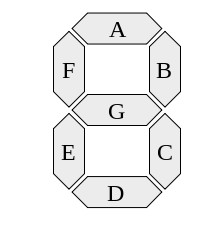
\includegraphics[width=0.2\textwidth]{imgs/7seg-labels.png}
\end{center}
\vspace{-2em}
\caption{Ordre des segments. Crédit~: H2g2bob @ Wikipedia}
\label{fig:segorder}
\vspace{-2em}
\end{wrapfigure}

Le programme ne prend aucun argument. Il attend sur son entrée standard des caractères formatés comme la sortie du processeur (§\ref{ssec:compilo_io}), c'est-à-dire 16 caractères à la suite. Les caractères contrôlent chacun un afficheur, dans l'ordre \verb!--HHMMSSYYYYMMDD! respectivement heure à deux chiffres, minutes, secondes, année à 4 chiffres, mois, jour.

Les bits du caractère contrôlent les segments d'un afficheur, à savoir en commençant par les poids forts \verb!-gfedcba! (figure \ref{fig:segorder} ci-contre).

\subsection{Fonctionnement et optimisations}

La lecture de l'entrée standard est gérée dans un thread séparé du thread principal, se chargeant de l'affichage~; la communication entre threads est aisée puisque l'un est en écriture seule sur la mémoire partagée quand l'autre est en lecture seule.

Le thread d'affichage est volontairement limité à 30 FPS~: 30 fois par seconde, il demande au thread de lecture des valeurs pour chacun de ses segments et met à jour son interface. Ceci fut une première amélioration notable des performances, par rapport à un modèle où les segments sont rafraîchis aussi vite que possible.

Le thread de lecture, quant à lui, a été bien plus optimisé. Les modèles suivants ont été considérés, successivement~:
\begin{itemize}
\item Lorsque des valeurs sont demandées, on lit 16 caractères sur \lstc{stdin}~; lorsque le rafraîchissement est terminé, on \lstc{fflush} l'entrée standard afin d'ignorer ce qui est arrivé pendant ce temps. Cette option n'a jamais fonctionné, d'autant qu'elle ferait perdre tout repère de \og début de bloc de 16 caractères \fg{}.

\item On lit en continu des blocs de 16 caractères et, à chaque demande de rafraîchissement, on renvoie les 16 derniers acquis. Cette option marchait bien, mais était trop lente.

\item La \og boucle infinie \fg{} de lecture étant gérée avec Qt, le modèle signal/slot impose de faire en réalité une fonction de lecture se terminant par l'empilement d'un événement \og appeler la fonction de lecture \fg{}. Cette procédure est très coûteuse (beaucoup plus que \lstc{getchar}~!). Ainsi nous ignorons systématiquement 12 blocs sur 13~: la fonction de lecture lit $13 \times 16$ caractères et ne conserve que les 16 derniers. La fréquence de notre processeur nous permet (et nous oblige) à procéder de la sorte pour avoir une vitesse d'affichage raisonnable.
\end{itemize}

Avec ce fonctionnement, nous arrivons à une horloge capable de supporter l'entrée massive qui lui est fournie chaque seconde, sans ralentir le système global.

\end{document}